\documentclass[a4paper, twocolumn]{article}
\usepackage{dblfloatfix}
\usepackage{url}
\usepackage[utf8]{inputenc}
\usepackage[english]{babel}
\usepackage[T1]{fontenc}
\usepackage{color}
\usepackage{amsmath}
\usepackage{amsfonts}
\usepackage{amssymb}
\usepackage{graphicx}
\usepackage{placeins}
\usepackage[toc,page]{appendix}
\usepackage{tikz}
\usetikzlibrary{positioning,shapes}
\usepackage{pgfplots}
\usepackage[font=small,labelfont=bf,tableposition=top]{caption}
\usepackage{cuted}
\usepackage{tocloft}% http://ctan.org/pkg/tocloft

%%%%%%%%%%% Numerotation
\renewcommand{\thesection}{\Roman{section}.}
\renewcommand{\thesubsection}{\Roman{section}.\arabic{subsection}.}
\renewcommand{\thesubsubsection}{\Roman{section}.\arabic{subsection}.\alph{subsubsection}.}
\setlength{\cftsecnumwidth}{2em}% Set length of number width in ToC for \subsection
%%%%%%%%%%%

%%%%%%%%%%%%%%%%%%%%%% Sizes
\newcommand{\changeSize}[1]{\fontsize{#1pt}{7.2}\selectfont}
\newcommand{\tinySize}{\changeSize{8}}
\newcommand{\smallSize}{\changeSize{12}}
\newcommand{\normalSize}{\changeSize{16}}
\newcommand{\bigSize}{\changeSize{22}}
\newcommand{\hugeSize}{\changeSize{30}}
%%%%%%%%%%%%%%%%%%%%%%

%%%%%%%%%%%%%%%%%%%%%% Colors
\definecolor{DiagramBlue}{HTML}{00B4E9}
\definecolor{DiagramOrange}{HTML}{F8CA37}
%%%%%%%%%%%%%%%%%%%%%%

%%%%%%%%%%%%%%%%%%%%%% Itemize bullet-point
\renewcommand\labelitemi{--}
%%%%%%%%%%%%%%%%%%%%%%

%%%%%%%%%%%%%%%%%%%%%% Tikz legend
% argument #1: any options
\newenvironment{customlegend}[1][]{%
    \begingroup
    % inits/clears the lists (which might be populated from previous
    % axes):
    \csname pgfplots@init@cleared@structures\endcsname
    \pgfplotsset{#1}%
}{%
    % draws the legend:
    \csname pgfplots@createlegend\endcsname
    \endgroup
}%
%%%%%%%%%%%%%%%%%%%%%%

% makes \addlegendimage available (typically only available within an
% axis environment):
\def\addlegendimage{\csname pgfplots@addlegendimage\endcsname}

\title{Object Recognition and People Tracking in a home environment}
\author{Ismail Lahkim Bennani}

\date{\today}


\begin{document}
    \twocolumn[{\begin{@twocolumnfalse}
		\maketitle
        \tableofcontents

        \vspace{2em}
	\end{@twocolumnfalse}}]

    \begin{figure}[!b]
        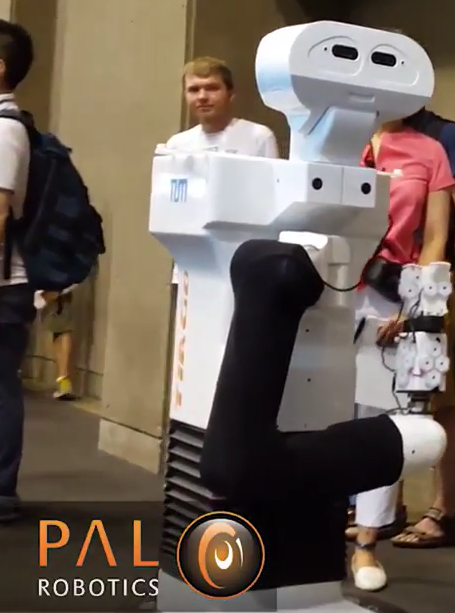
\includegraphics[width=\columnwidth]{../img/tiago.png}
        \caption{Our robot, Tiago}
        \label{tiago}
    \end{figure}

    \section*{Introduction}
    
    Currently, object detection, recognition and tracking are three of the most important problems of computer vision. 
    
    Deep learning methods give astonishing results in object recognition but they require training and they cannot detect unknown objects whereas other methods without neural networks are not yet satisfying enough. 
    
    Concerning object tracking, we know some very accurate solutions for fixed cameras but we still have a lot of trouble when the camera is moving.
    
    For my M1 internship, I was at ICS (Institute for Cognitive Systems) in Munich. I stayed there for 5 months and my main work was about object recognition and people tracking using a camera mounted on a robot's head. The robot we used was Tiago (see Fig. \ref{tiago}), it was lent by PAL Robotics to ICS in order to compete in the Robocup@Home2017\footnote{http://www.robocupathome.org} competition. The Robocup@Home competition is the largest international annual competition for autonomous service robots. It consists in several challenges that take place in arenas that are built like normal apartments.
    
    My supervisor offered me to join a team of 3 master students, 2 PHD student and 2 researchers (that later became a team of 7 master students, 2 PHD students and 3 researchers) to work on the Robocup@Home project and I agreed, I've been working with them for 4 months and we went to Nagoya, Japan to compete. Before I joined the team, I worked on object recognition with the Hololens\footnote{https://www.microsoft.com/hololens}, a pair of augmented reality glasses made by Microsoft.
    
    The result of my internship is the python code I wrote that will soon be released on github, it is basically a set of tools to do object detection, recognition and tracking using an RGB(D) camera. It relies a lot on the scikit-learn \cite{scikit-learn} and opencv \cite{itseez2015opencv} libraries.
    
    First of all, I will present my work through two of the challenges we had to complete for the competition, then I will briefly talk about my work with the Hololens.

    \section{Challenge 1: Storing groceries}

        This test focuses on the detection and recognition of objects and their features, as well as object manipulation. This is the scenario as described by the rulebook \cite{rulebook2017}.\\

    \paragraph{Setup} The challenge takes place in a kitchen, there are at least a cupboard with some objects on it and a table with at most 10 objects on it. The robot starts facing the cupboard, the starting position is not specified, the table is less than 2 meters away from the cupboard. Their is one door on the cupboard, covering at most half of it. The objects on the cupboard and on the table can be "known" objects, "alike" objects or "unknown" objects. Some objects are given to the teams the day before the challenge, those are the "known" objects. The "alike" objects are objects that resembles "known" objects (for example, a bottle of coke and a bottle of water). The "unknown" objects are objects that are completely different.

    \paragraph{Task} The robot must start by opening the door, it can ask the referee to do it instead. Then it should look at the cupboard and identify the objects on it. Then it has to find the table, go to the table and identify the objects on it. Then it has to grasp on of the object and place it on the cupboard. It should allocate similar objects together (bottles should go with bottles on the cupboard) as much as possible. Then it has to go back to the table and start again, until there are no more objects on the table.
    
    For this challenge I worked on the object recognition programs.

    \subsection{Object recognition}

    The core component of the perception module is the one used for object recognition. We do that by using two complementary approaches: a deep convolutional network called YOLO\cite{redmon2016yolo9000} and a clustering of the objects based on our depth image.

  YOLO is powerful at discriminating between a wide range of objects given a proper dataset while the depth-based approach doesn't need any training.

  The combination of these two methods give use a robust way of finding  known and unknown objects in an RGB-D image. We can then use the 2D information we get from the recognition to find the position and size of the objects in the real world.

    \subsubsection{YOLO}

    YOLO (and more specifically YOLOv2) is considered as one of the most performing neural network for object recognition. It was used by 12 out of 15 teams in RoboCup@Home2017 and by more than half of the teams in all the RoboCup competitions. It takes an image as input and outputs labelled bounding boxes corresponding to the recognized objects (see Fig. \ref{YOLO_rgb})

    \begin{figure}
        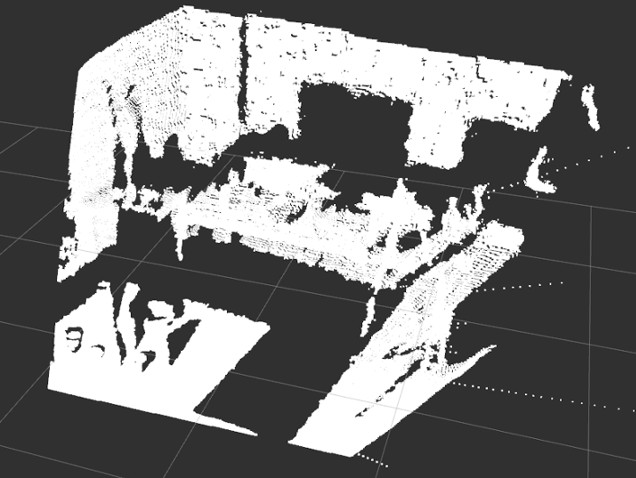
\includegraphics[width=\columnwidth]{../img/table_pcl.jpg}
        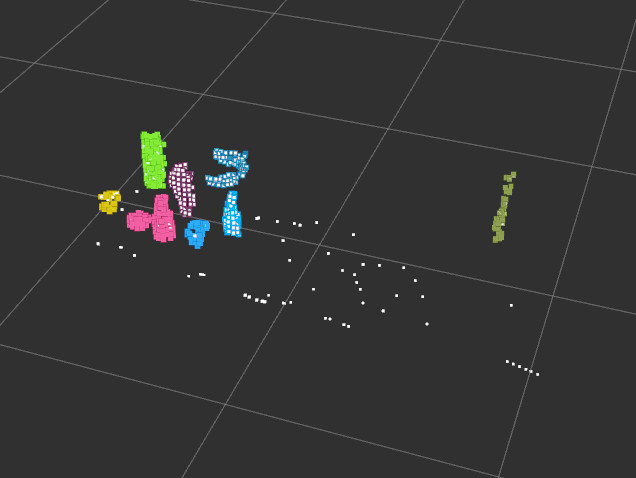
\includegraphics[width=\columnwidth]{../img/cluster_obj_pcl.jpg}
        \caption{Point cloud (top) and object clusters on the table (bottom)}
        \label{pcl_clust}
    \end{figure}

    We decided to implement our perception module in python but YOLO has been implemented by it's author in C. I found several other implementations in python using either caffe or tensorflow but none of them was as fast as the original version. The C version was 5 to 10 times faster than the others, therefore I decided to create a bridge between YOLO and the rest of the code. Concretely, the python class I created spawns a new process to run YOLO and communicates with it through pipes.

    I used a Nvidia GTX 1060 for my tests, the original YOLO can process an image in 100 to 150 milliseconds while the python class does it in 110 to 180 milliseconds.

    However, this approach has two major problems. One of our biggest constraints was processing power: our robot had no graphic card therefore we couldn't use it to run a deep neural network. We had to use an external computer mounted on the robot to do our computations. At first we wanted to build a desktop-like computer for this purpose but we realised that it would be too difficult to cool the components in such a small space, and most importantly that it would be nearly impossible to power it. We were not allowed by the company that lent us the robot to use its batteries to power anything else than the robot itself and we didn't have enough room to put a battery big enough to power a computer powerful enough for our purposes without using custom components. We decided to use a laptop computer and the most powerful we had was using an Nvidia GTX 1060.

    The second major problem is that YOLO is not able to recognize objects that were not part of the training dataset. For this challenge we had to be able to find unknown objects, i.e. objects that we discover during the challenge.

    \subsubsection{Depth clusters}

    To solve the unknown objects problem, we decided to use the depth point cloud that we get from our depth camera to recognize every potential object in our field of view.

    To do so we start by removing the points that are not in front of us and by removing all the big planar components from our point cloud, that corresponds to the floor, the walls, the tables etc.. Then we cluster the remaining points by Euclidean distance i.e. two points are clustered together if they are close enough to each other (see Fig. \ref{pcl_clust}). The threshold used in Fig. \ref{pcl_clust} is 2cm, that means that two points are considered to be part of the same object (cluster) if they are less than 2cm apart from each other. Finally we compute the 2D projection of each cluster on the RGB image to get a bounding box of the unknown object (see Fig. \ref{rgb_clust}) using the projection matrices that we get from the robot.

    In practice, we could only use this method to find the objects on a table when we were looking at the table. When we were looking at the shelf for example, we had too many wrong predictions: the rims of the shelf were unknown objects, some pieces of the wall were not big enough on the point cloud (because of partial occlusion of the wall by other objects) to be removed as big planes, therefore they were objects too. However, that was not a big issue since we only care about the unknown objects for grasping them, and in our scenario those objects are on a table.
    
    \begin{figure}[!b]
        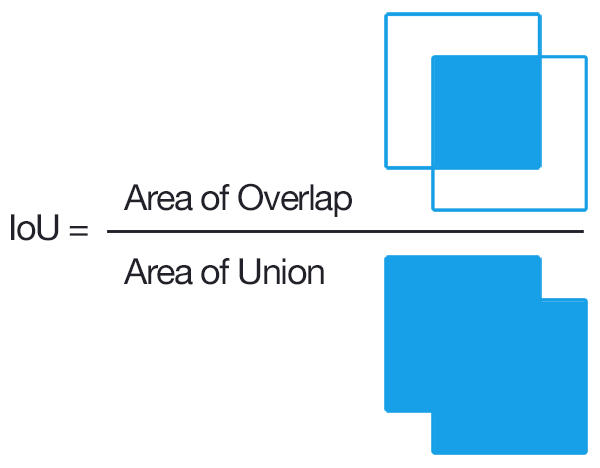
\includegraphics[width=\columnwidth]{../img/iou_equation.png}
        \caption{Intersection over Union (IoU)}
        \label{IoU}
    \end{figure}

    With this method we find most of the objects on the scene, even those that YOLO recognizes. We need to merge the two approaches results together, to do so we compare each couple of predictions (one from YOLO, the other from the depth image) and we compute the intersection over union of the area of their bounding box. The intersection over union (see Fig. \ref{IoU}) is an evaluation metric often used in object detection, here I use it to determine if two detections are the same or not. If the result is close enough to 1, it's the same detection (see Fig. \ref{recognition_rgb}).

    \begin{figure}
        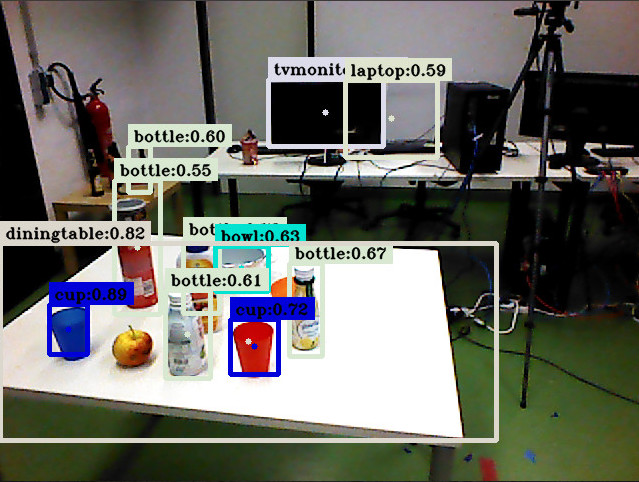
\includegraphics[width=\columnwidth]{../img/yolo_table.jpg}
        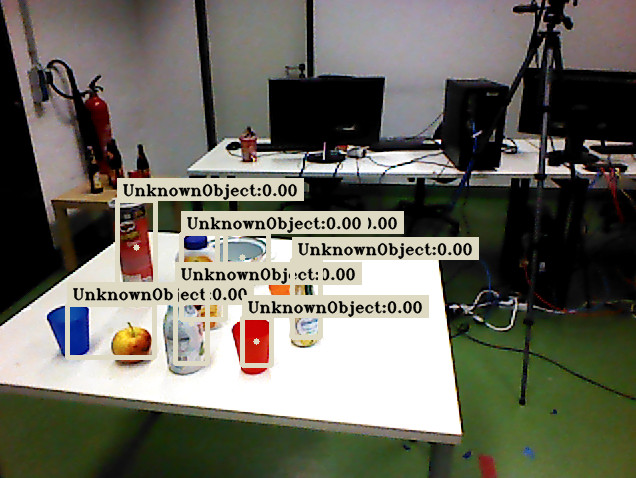
\includegraphics[width=\columnwidth]{../img/cluster_obj_rgb.jpg}
        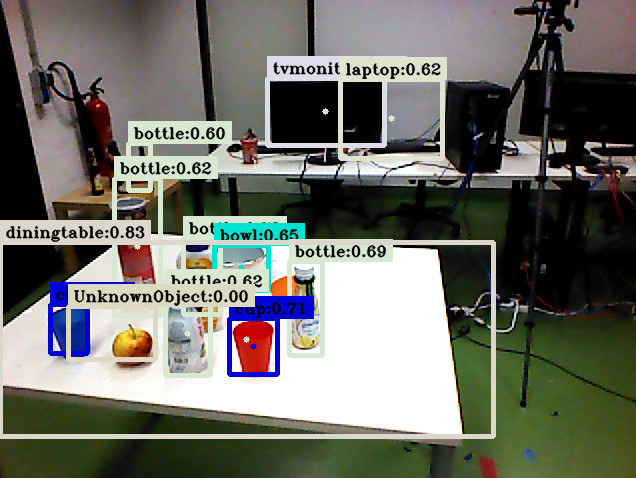
\includegraphics[width=\columnwidth]{../img/summary_recognition.jpg}
        \caption{YOLO predictions (top), predictions from depth clusters (middle) and the final predictions (bottom)}
        \label{YOLO_rgb}
        \label{rgb_clust}
        \label{recognition_rgb}
    \end{figure}

    This method was first intended to find the unknown objects in this challenge, but we realised that we could also use it to enhance our recognition. I added an extra step to this approach: classification. Once we get the 2D bounding box in the RGB image, we compute a color histogram of the object's image and we run it through an SVM to identify it. The SVM is trained beforehand with the known objects that we had the day before the challenge.

    \subsection{From 2D to 3D}

    Once we have our 2D bounding boxes, we need to find the position of the objects in the world to be able to interact with them. We use the depth image for that (see Fig. \ref{depth_image}).

    \begin{figure}[!b]
        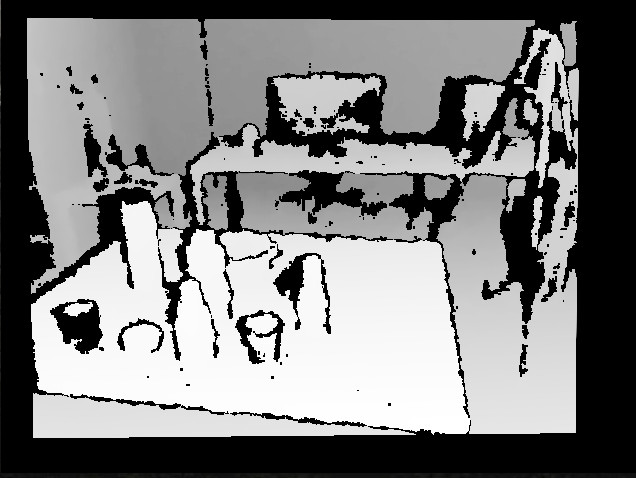
\includegraphics[width=\columnwidth]{../img/depth_image.jpg}
        \caption{Depth image}
        \label{depth_image}
    \end{figure}

    The depth image is a float32 matrix where each cell is the depth of the corresponding pixel with respect to the camera (located in the robot's head). Given a 2D bounding box, we crop the original depth image to get the part corresponding to the object, we compute a histogram of the depth values and we down sample it to 5cm wide bins, then we select the bin that contains the most points. This method is a lot more robust than taking the depth of a single pixel in the bounding box (our first solution was to take the depth value of the pixel in the center of the bounding box). We can see in Fig. \ref{depth_image} that the leftmost cup is almost black in the depth image, a black pixel means that we don't have any depth value for that pixel and that happens a lot with transparent or semi-transparent objects. If we use the value of the pixel in the center of the bounding box we would get a depth equal to NaN, with the histogram method we get the depth of some point on the object.

    \begin{figure*}[!b]
        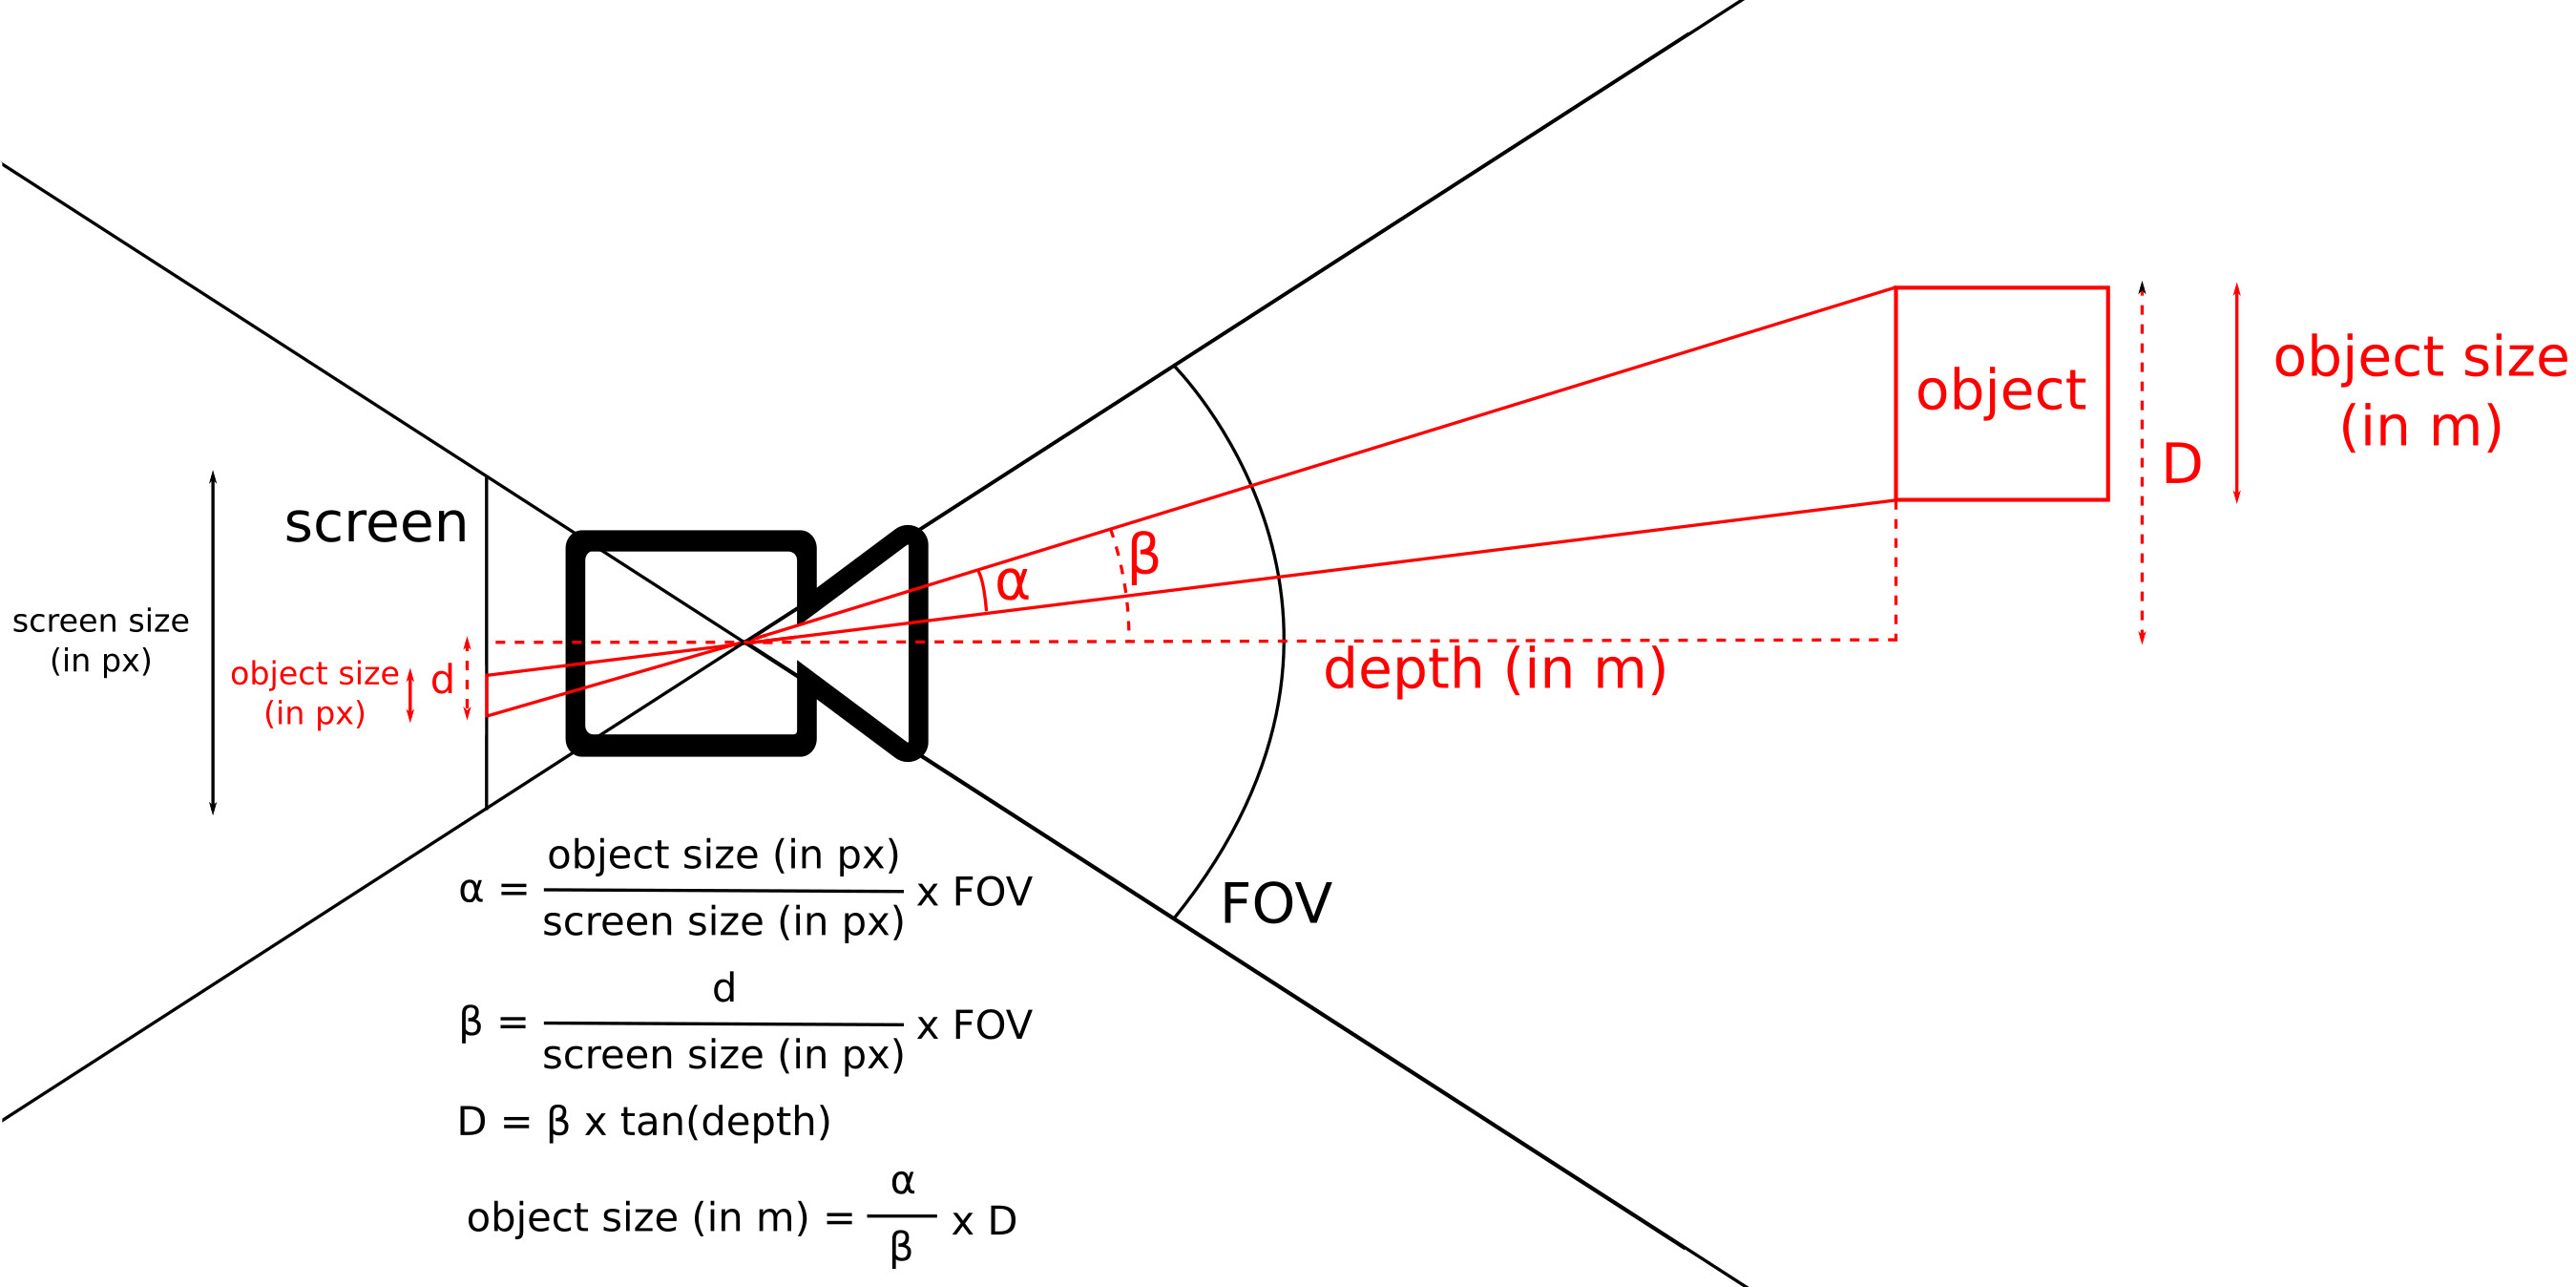
\includegraphics[width=\textwidth]{../img/camera_size.jpg}
        \caption{Compute the size of the object with the depth information}
        \label{camera_size}
    \end{figure*}

    We can also estimate the apparent size of an object with the informations we have. We compute the size ratio of the bounding box to the size of the image, then with the horizontal and vertical field of view of the camera we can compute the angular size of the object in the image with respect to the camera and we can find the actual size of the object thanks to it's depth relative to the camera (see Fig. \ref{camera_size}). With this method we find the apparent width and height of the object, we cannot find its third dimension but we don't need it.

    The size we compute is a rough approximation (I'm approximately 1.77m tall and the recognition gives me a height of approximately 1.60m) but we don't really need a high precision: the size is used to find what object is graspable based on the maximal width of our robot's gripper, it is not used for the actual grasp. 
    
    For the actual grasp, the robot uses an artificial skin \cite{hum} developed by ICS\footnote{https://www.ics.ei.tum.de}. The skin has several sensors such as a pressure sensor, a thermometer, a proximity sensor etc.. The robot moves the gripper toward the position given by the perception module and we use the proximity sensors and the pressure sensors in the skin cells to adjust the gripper's position and size to the object's actual position and size.
    
    \begin{figure*}
        \resizebox{.9\textwidth}{!}{\centering{
  \begin{tikzpicture}
    [node distance=4cm,
     plain/.style={},
     node/.style={draw, rectangle, outer sep=.1cm, inner sep=.5cm},
     topic/.style={draw, dashed, ellipse, outer sep=.1cm},
     service/.style={draw, dashed, rectangle, outer sep=.1cm},
     picture/.style={}]

    \node[node] (n_0) {recognition\_server};
    \node[node] (n_1) [above=.6cm of n_0] {YOLO\cite{redmon2016yolo9000}};
    \node[topic] (t_0) [below of=n_0] {/recognition/bb2D};
    \node[plain] (p_1) [right=0cm of t_0] {2D Bboxes};
    \node[node] (n_2) [below of=t_0] {from2Dto3D};
    \node[topic] (t_1) [below of=n_2] {/recognition};
    \node[plain] (p_2) [right=0cm of t_1] {3D points};

    \node[topic] (t_2) [left=1cm of n_0] {/recognition/bb2D/unlabeled};
    \node[plain] (p_3) [above=0cm of t_2] {unlabeled 2D bounding boxes};
    \node[node] (n_3) [left=1cm of t_2] {\begin{tabular}{c}classifier\\\smallSize(SURF, COLOR)\end{tabular}};
    \node[node] (n_4) [left=1cm of n_3] {cluster\_objects};

    \node[plain] (p_0) [above=.5cm of p_3] {sensors};

    \node[picture] (pic_0) [below right=0cm and -6.5cm of n_3] {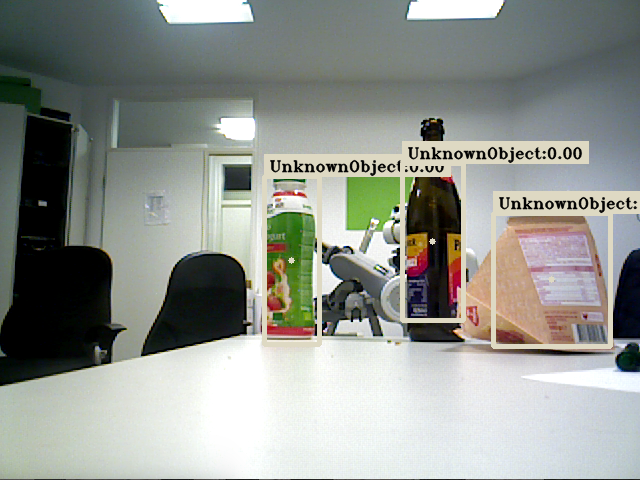
\includegraphics[width=7cm]{../img/cluster_objects.png}};
    \node[picture] (pic_1) [right=0cm of pic_0] {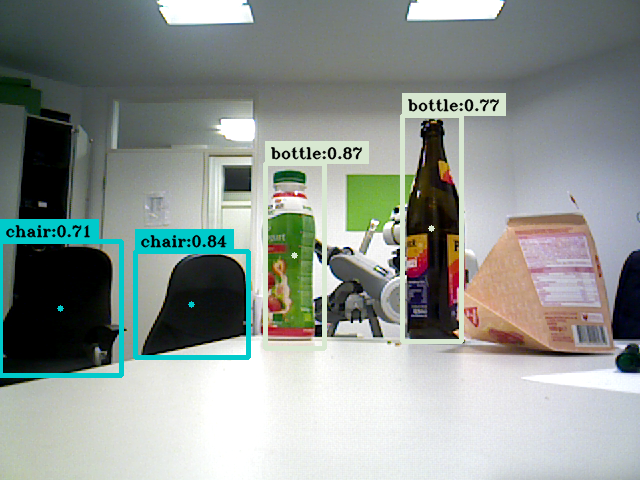
\includegraphics[width=7cm]{../img/YOLO.png}};
    \node[picture] (pic_2) [below right=0cm and -5cm of pic_0] {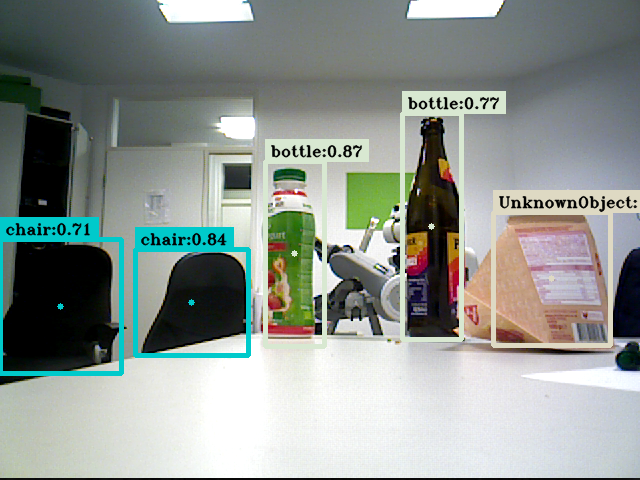
\includegraphics[width=10cm]{../img/recognition.png}};

    \node[plain] (label_0) [above left=-1.5cm and -4.2cm of pic_0] {\small\color{white} cluster\_objects};
    \node[plain] (label_1) [above left=-1.5cm and -2.0cm of pic_1] {\small\color{white} YOLO};
    \node[plain] (label_2) [above left=-1.5cm and -5.0cm of pic_2] {\small\color{white} recognition\_server};

    \draw [->]
      (n_1) edge (n_0)
      (n_0) edge (t_0)
      (t_0) edge (n_2)
      (n_2) edge (t_1)
      (n_3) edge (t_2)
      (t_2) edge (n_0)
      (n_4) edge (n_3)
      (p_0) edge (p_0-|n_1.west);

    \draw [->, to path={-| (\tikztotarget)}]
      (p_0) edge (n_4);

    \begin{customlegend}[legend entries={nodes, topics},
                         legend style={at={(5, 2.2)},anchor=center}]
      \addlegendimage{black, area legend}
      \addlegendimage{black, area legend, dashed}
    \end{customlegend}

  \end{tikzpicture}
}
}
        \caption{Recognition module}
        \label{recognition_module}
    \end{figure*}

    The final result of the recognition module (see Fig. \ref{recognition_module}) is the label, position and size of each recognized object relative to a fixed coordinate frame (see Fig. \ref{recognition_result}).

    \begin{figure}
        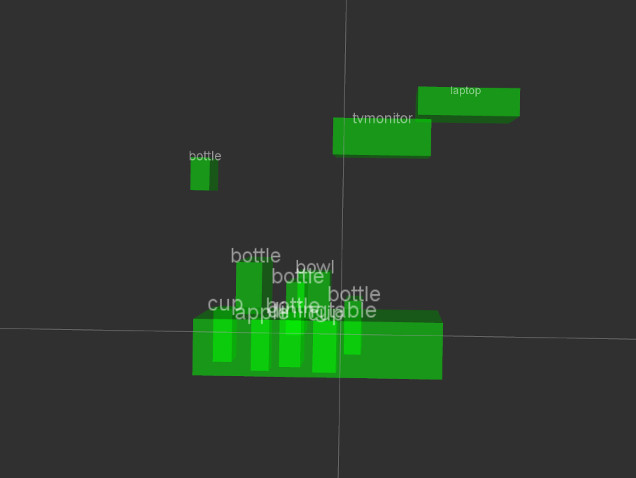
\includegraphics[width=\columnwidth]{../img/recog_markers.jpg}
        \caption{Recognition result}
        \label{recognition_result}
    \end{figure}

    \subsection{Results}

    Our method for solving the challenge is the following. Note that we had some time before the challenge to map the room and to set some predefined positions. It was not specified in the rulebook but they told us before the challenge that we could do it.
    \begin{enumerate}
        \item Go in front of the shelf
        \item Ask the operator to open the door
        \item Recognize the objects in the shelf for some frames and keep the stable detections (sometimes we have noise in the recognition). A detection is stable if it appears approximately at the same position for several consecutive frames
        \item Cluster the objects in the shelf based on their semantic class and their position (if we have a cup and a bowl next to each other, that part of the cupboard is the part where we should place containers)
        \item Compute available empty space next to each cluster (we do that with the depth image, if the space is empty, the depth value of the corresponding pixel is significantly bigger than the depth value of the closest objects)
        \item Go to the table
        \item Recognize the objects in the table for some frames and keep the stable detections
        \item Choose an object to grasp and grasp it: the choice is based on the object itself (a bottle is easier to grasp than a bowl), the object position (start with the closest ones to avoid collisions) and the clusters found in the shelf (don't grasp an object if you don't know where to put it)
        \item Go back to the shelf
        \item Compute a proper placing position: the choice is based on the empty space computed before.
        \item Place the object
        \item Repeat from step 6 until there are no more objects on the table
    \end{enumerate}

    The main problem we encountered during the competition was the time it took us to perform the task. We had 1:30 minutes to grasp the first object on the table, and it took us 1:35 minutes to do it, mainly because we lost too much time recognizing every object on the shelf (the shelf is too big to see everything in one picture, we had to move the robot's head several times, see Fig. \ref{shelf_recog}) and computing clusters and proper placing positions.

    This problem was common to all the team, actually there is only one team that managed to grasp the object in the given time but they couldn't place it in the shelf, we managed to get the third place (out of 15) thanks to the objects we recognized on the shelf. The day after the challenge, we worked on reducing the delays (the 1:30 minute rules was not part of the original rulebook, it was added 1 hour before the actual challenge) and we managed to grasp and place 1 object in the given time.

    \begin{figure}
        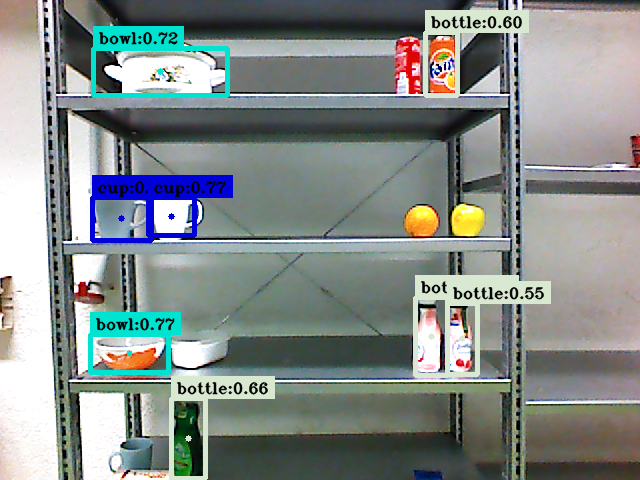
\includegraphics[width=\columnwidth]{../img/yolo_shelf.png}
        \caption{Shelf objects recognition}
        \label{shelf_recog}
    \end{figure}

    \section{Challenge 2: Help me carry}

    This test focuses on safe, robust navigation, people following and navigation in unknown environments. This is the scenario as described by the rulebook \cite{rulebook2017}.\\

    \paragraph{Setup} The challenge takes place in the arena and outside of it, the robot starts waiting at a random location in the arena. There is a car somewhere outside the arena and several bags with groceries next to it. A professional operator is selected to act as the operator of the robot. There are no restrictions on other people walking by or standing around outside of the arena.

    \paragraph{Task} The robot should wait for the operator to say "follow me", then it should memorize the operator. The robot may ask the operator to perform some setup procedure. When the robot is ready, it should start following the operator who should start walking, in a natural way, towards the car. When they reach their goal, the operator will indicate the robot that they arrived, then they will give it a bag of groceries. The robot should bring the bag to a specific location inside the arena.

    For this challenge I used the previous work to recognize people and I worked on the tracking programs.

    \subsection{Tracker module}

    Since our Object Recognition module is able to detect people as any other object, we use it as our people detector for the tracker. The deep neural network that we use is very good at finding people, it can even recognize the reflection of a person on a semi-reflective surface such as a monitor.

    However, we want to do more than detection, we want to track. For that we need to match all the detections of people that we have between the frames. We do that by considering our problem as a stable marriage problem \cite{gale62a}. In addition to that, we need to identify the people that we see as "operator" or "not operator" to solve the occlusion problem for example, or to detect that we don't see our operator anymore.
    Our approach to solving this problem is to use feature descriptors such as color histograms and SVMs \cite{Cortes1995}. 

    \subsubsection{Stable marriage problem}

    \paragraph{Definition} The stable marriage problem is the problem of finding a stable matching between two equally sized sets of elements given an ordering of preferences for each element.

    A \textit{matching} between two sets $A$ and $B$ is a mapping from the elements from $A$ to the elements from $B$. A matching is \emph{not} stable if:
    \begin{itemize}
        \item There is an element $a$ of the first matched set which prefers some given element $b$ of the second matched set over the element to which $a$ is already matched, and
        \item $b$ also prefers $a$ over the element to which $b$ is already matched.
    \end{itemize}

    In other words, a matching is stable if we cannot find two couples in $A \times B$ in which two of the elements would rather be together than with their respective partners.

    \paragraph{Implementation} In our case, we want to match the people detections from frame $n-1$ to the people detections from frame $n$. Our elements are the detections and we use the 3D euclidean distance between the position of the people we detect (that we get from the recognition module) to order the elements. The closer they are to each other, the more likely they correspond to the same person.

    \begin{figure}
        \centering
        \begin{tikzpicture}
          \node (10) {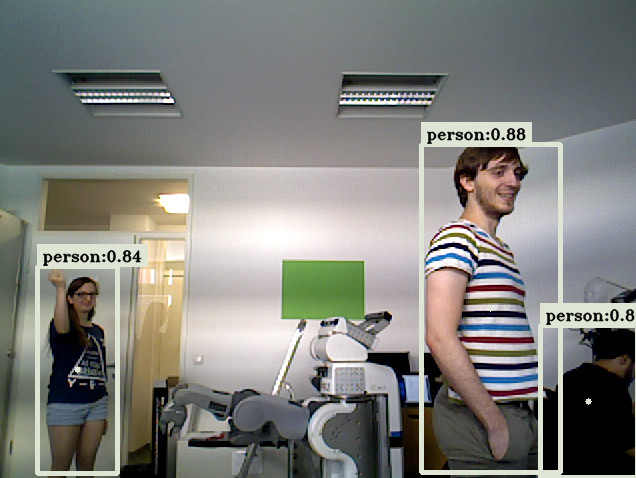
\includegraphics[width=\columnwidth]{../img/tracker_people_det1.jpg}};
          \node (11) [above left = -.7cm and -2.1cm of 10] {\color{white}Past frame};
          \node (20) [below = 0cm of 10] {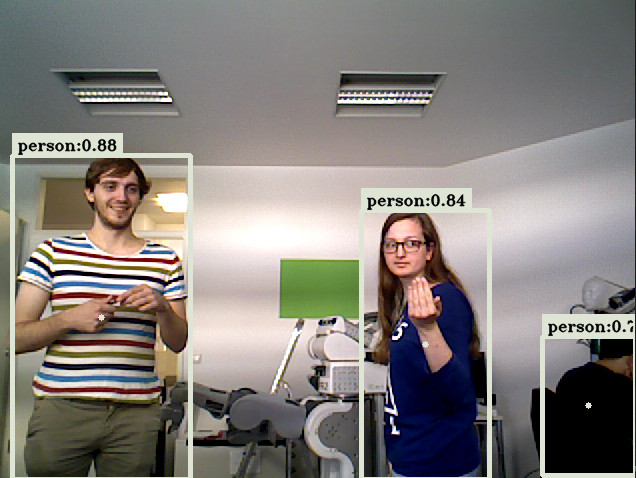
\includegraphics[width=\columnwidth]{../img/tracker_people_det2.jpg}};
          \node (21) [above left = -.7cm and -2.55cm of 20] {\color{white}Current frame};
          \node (30) [below = 0cm of 20] {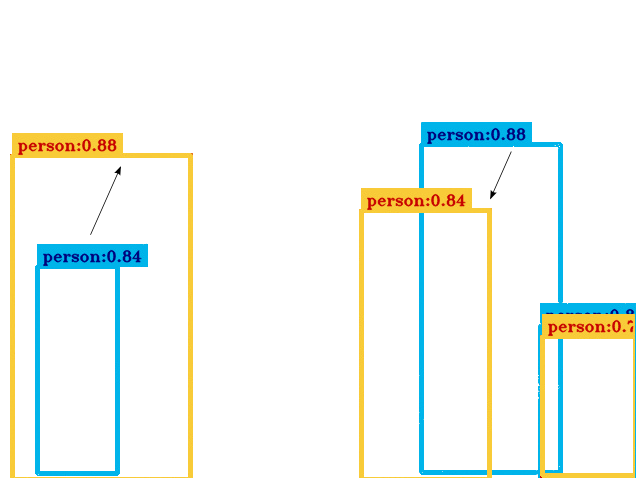
\includegraphics[width=\columnwidth]{../img/pred_bboxes.png}};
          \node[rectangle, draw, minimum width=4cm, minimum height=2cm] (0) [below=0cm of 30] {};
          \node[rectangle, draw, fill=DiagramBlue, minimum width=1cm, minimum height=.55cm] (1) [above left=-.85cm and -1.2cm of 0] {};
          \node[rectangle, draw, fill=DiagramOrange, minimum width=1cm, minimum height=.55cm] (2) [above left=-1.7cm and -1.2cm of 0] {};
          \node (3) [right=0cm of 1] {\tinySize past detections};
          \node (4) [right=0cm of 2] {\tinySize current detections};
        \end{tikzpicture}
        \caption{Detections matching}
        \label{pred_match}
    \end{figure}

    To solve this problem I used the Gale-Shapley algorithm \cite{10.2307/2312726} that always give a stable match with a quadratic complexity. In our case, the complexity is quadratic with respect to the number of past people detections that is usually small (even with a crowd of people we won't detect more than $n \approx 100$ people, i.e. $n^2 \approx 10 000$ elementary computations which is fairly small).

    But the problem here if that our two sets of detections is not necessarily equally sized: what if someone appears or disappears in our new frame. To solve this, I made the previous algorithm stop whenever one of the two sets is exhausted. We are then left with one possibly non-empty set, if it is the past detections one, it means that the remaining people have disappeared, if it is the current detections one, it means that the remaining people have appeared.

    Thanks to this algorithm we update an environment of people that we see and we track them all from one frame to the other. Given the operator's detection at one frame, we can keep track of their position as long as there are people in our field of view under the assumption that those people don't move too much from one frame to the other. You can see the result of the algorithm on an example in Fig. \ref{pred_match}. If we ignore the RGB image and only take into account the bounding boxes, the algorithm finds a very good solution.

    However, this is not enough. Our assumption is too strong, we get the detections at an approximative rate of 5 FPS, it is slow enough for a person to get lost in a crowd. And more importantly, we did not address one of the most difficult problem of tracking: occlusions. What if someone passes in front of our subject ? Well, with this method if at some point one person is fully occluded by the other (which means that the people detector only sees one person in the frame instead of two), the person in front would become our new operator, no matter if they are the right one or not.

    \paragraph{Enhancement} Until now, the only parameter we took into account for tracking is the positions of our subjects with respect to the camera. To address the issue mentioned above, we decided to consider the movement of the subjects. Instead of using the position of the past detections to find a matching, we use a Kalman filter \cite{kalman} to estimate the next position of each subject given their previous positions. A Kalman filter is an algorithm that uses a series of measurements observed over time, containing statistical noise and other inaccuracies, and produces estimates of unknown variables (in our case, the 3D position of the person). We run the Gale-Shapley algorithm with these estimations, find the matching and correct each Kalman filter with the new position of the subject they are tracking. In addition to that, we added a lifespan to each person in our environment, this lifespan is set to some default value (typically 10 frames, i.e. 2 seconds) each time the person is detected on the image, and decreased each time the person is not detected. Once it reaches 0, the person is considered lost and is deleted from the environment. When two people occlude each other in the RGB image, they have the same 2D projection but they don't have the same 3D position and more importantly they don't have the same trajectory. When we go from 2 detections on the image to one detection, the person that disappeared is not lost, it stays in the environment and we keep estimating their probable location with their Kalman filter until they reappear or until it is too late.\\

    With this enhancement, we managed to have pretty good results in simple scenarios, with a fixed camera and a small number of people on screen (3 to 4 in our tests). But as soon as the camera starts moving, we get more noise in our images (especially the depth image) and the 3D positions that we measure are not as precise as they were.

    \subsubsection{Election manager}
    
    Until now, the only information we used is the position of the detection in our world, which is basically what the depth camera gives us. We can see on Fig. \ref{pred_match} that it is not enough, if the people move too much between two frames, our result are wrong. To improve the result, we decided to use the RGB camera too: we try to use an SVM to recognize our operator amongst all the detections.
    
    \paragraph{Training set} At the very beginning of the challenge, we ask our operator to rotate in front of the robot therefore we can gather some positive samples. We require that there is no other person close to the robot in its field of view during that phase, to avoid any false positive (we typically gather 60 positive samples). Once it is done, we use some predefined samples that we gathered at our lab ourselves with the same camera as negative samples. Those negative samples are pictures of several people (6 different people) wearing different clothes (with different colors) under different light conditions (natural light, artificial light, different light intensity, different time of the day etc..). We pick a given amount of negative samples (typically twice the number of positive samples) randomly from those images.
    
    \paragraph{Feature descriptors} We wanted to use several feature descriptors to learn the operator: color histograms are relevant in our case since the operator is not likely to change their clothes during the challenge but it is not robust enough since we don't know anything about the light condition throughout the challenge, therefore we decided to use SURF descriptors \cite{BAY2008346} as well. 
    
    I tried to look into LOMO\cite{2014arXiv1406.4216L}, a feature descriptor for person re-identification, I implemented the feature extraction (and some auxiliary functions) in python (I used the matlab code provided by the authors as a base-line) but I didn't have enough time to test it properly therefore I didn't use it for the competition.
    
    \paragraph{Election} Once we have our dataset, we train several SVMs, one per feature descriptor. If the feature extractor does not output a fixed-length vector, we have to find another way to represent the data or else we cannot train the SVM. For SURF, we use the k-means algorithm to construct a bag of words with all the 64-dim vectors from the positive and negative set, and for each feature descriptor we compute the histogram of words (using k-means) which is a fixed-length vector (the size is the number of words, which is the number of clusters in k-means).
    
    Once we have our SVMs, for each new detection we compute the prediction of each SVM, which is a 1 or a 0 (operator or not operator) and the final result is the sum of all the predictions. We call this the election manager because each SVM approves or not one candidate and our goal is to elect the most wanted one as operator.
    
    The final result of the tracking module (see Fig. \ref{tracker_module}) is the position of the operator at each frame. The tracking pipeline is quite fast but we receive the frames at 5 FPS from the recognition module therefore the actual update speed is around 5 Hz.
    
    \subsection{Results}
    
    Our method to solving the challenge is the following.
    
    \begin{enumerate}
        \item Detect the people we see, the closest person to the center of the frame (in front of the robot) is the operator
        \item From now on, for each frame, run the stable marriage algorithm to keep track of the people we see. Each person have their own unique ID
        \item Start learning phase, ask the operator to rotate and to move a little bit in front of the robot to get samples from different angles and at different scales
        \item While learning, detect the operator and save the detection as positive sample (we learn for a given amount of frame, typically 60)
        \item Train the SVMs
        \item Start following, tell the operator you're ready to go
        \item For each frame, after the environment have been updated, run the election manager on each detection
        \begin{itemize}
            \item If no operator was found (the election manager answered 0 for every detection), don't change the operator ID
            \item Else, change the operator ID to the ID of the positive detection that is the closest to the previous operator's detection
        \end{itemize}
        \item If the operator ID is still in our environment of people we track (we still see the operator), output their position and start again from step 7. Else, we lost the operator, say that you lost the operator and stop.
    \end{enumerate}
    
    The main problem we had was that the operator and the person that was chosen to occlude the operator during the "follow me" part of the challenge were moving very slowly. Way too slowly compared to a "natural way" of walking. Once the operator was occluded, the robot continued to follow the Kalman filter's predictions for some frames, but the lifespan of the detection ended before we could see him again (the occlusion lasted for several second, and the occluding person was moving perpendicularly to the operator). We didn't expect them to be this slow, therefore our parameters were not adapted to the situation.
    
    \begin{figure*}
        \resizebox{\textwidth}{!}{\centering{
  \begin{tikzpicture}
    [node distance=2.5cm,
     plain/.style={},
     node/.style={draw, rectangle, outer sep=.1cm, inner sep=.5cm},
     topic/.style={draw, dashed, ellipse, outer sep=.1cm},
     service/.style={draw, dotted, rectangle, outer sep=.1cm, inner sep=.5cm},
     picture/.style={}]

    \node[topic]   (t_0)                    {/recognition};
    \node[plain]   (p_0) [above=0cm of t_0] {3D points};
    \node[node]    (n_0) [below of=t_0]     {\begin{tabular}{c}person\_manager\\\smallSize Stable marriage\end{tabular}};
    \node[service] (s_0) [below left=-2.8cm and 2cm of n_0]  {
    \begin{tikzpicture}[every node/.style={minimum size=0cm, outer sep=.1cm, inner sep=.1cm},
                        small_node/.style={minimum size=0cm, outer sep=0cm, inner sep=0cm}]
      \node (0) {election\_server};

      \node             (10) [below=0cm of 0]   {\smallSize RGB images};
      \node             (11) [below=.5cm of 10] {\smallSize Feature extractor};
      \node[small_node] (12) [below=0cm of 11]  {\smallSize \textbf{SURF, COLOR, LOMO}};
      \node             (13) [below=.5cm of 12] {\smallSize Classifier};
      \node[small_node] (14) [below=0cm of 13]  {\smallSize \textbf{SVM}};

      \draw[->]
        (10) edge (11)
        (12) edge (13);

    \end{tikzpicture}
    };

    \node[topic]   (t_1) [below of=n_0]     {/tracking};
    \node[plain]   (p_0) [below=0cm of t_1] {3D point};

    \draw[->]
      (t_0) edge (n_0)
      (n_0) edge (t_1);

    \draw [<->]
      (n_0) edge (n_0-|s_0.east);

    \begin{customlegend}[legend entries={node, topic, service},
                         legend style={at={(-8,.5)},anchor=center}]
      \addlegendimage{black, area legend}
      \addlegendimage{black, area legend, dashed}
      \addlegendimage{black, area legend, dotted}
    \end{customlegend}

  \end{tikzpicture}
}
}
        \caption{Tracking module}
        \label{tracker_module}
    \end{figure*}
    
    \section{FORHD: Face and Object Recognition on a Holographic Device}
    
    FORHD is the name of the Hololens application I developed. I worked on this application before I started working on the Robocup@Home project and it was during this time that I came up with the architecture of the perception module. At the end of my internship, I updated the server-side of the application to make it use the new perception module. Since I was using a very similar interface than before, it took me a fairly small amount of time.
    
    The object recognition is based on YOLO, the same convolutional neural network used with Tiago. It needs a graphic card to run in real time therefore I had to use an external computer to do the computations. I decided to create a server on a desktop computer, the server would handle the object recognition part and will store an environment containing every object that we recognized. Then the Hololens would run a client that will send pictures to the server, compute the 3D position of the recognized objects and draw their bounding boxes as a hologram.
    
    \paragraph{Client-side}
    
    The client is the program running on the Hololens, it is the one that has access to the RGBD camera and that is interacting with the user. I wrote this program in unity, as advised by Microsoft on their website. They released a toolkit to help unity beginners to get started with the Hololens, that toolkit has, amongst other features, classes to handle the 3D mapping of the room we are in and some examples on how to do raycasts with unity. Raycasting is the tool I used to go from the 2D position of an object on the RGB image to its 3D position in the world.
    
    \paragraph{Server-side}
    
    The server is the program running on the desktop computer, it is the one that runs the perception module. It is an HTTP server waiting for requests. I created a small protocol for my application using GET, POST and PUT requests. For example, the client sends pictures and transformation matrices to the server with a PUT requests. I tried to do as much computations as I could on the computer since it is a lot more powerful than the Hololens.
    
    \paragraph{}
    The server is always waiting for requests, the only state it has is an environment of objects.
    The client main loop consists on sending pictures at a given rate. That rate is given by the server and is directly linked to the time it takes to process one image. Along with each picture, the client sends the current projection matrices (world coordinate frame to camera coordinate frame matrix and camera coordinate frame to picture coordinate frame matrix). For every picture it receives, the server will use the perception module to recognize objects on it, with the positions of the objects on the image and the projection matrices, it computes a 3D ray going from the camera position towards the object, the 3D ray of each recognized object is then sent back to the client. Then the client computes the position of the object by casting the 3D ray and looking for the first collision and sends the 3D positions (and size, we use the same method as seen in Fig. \ref{camera_size} to compute it) of all the objects to the server. The server updates its environment: if two points are too close to each other and have the same label (the distance threshold depends on the size of the object) then it is probably the same object. Then it answers with the new environment, the client will then draw that new environment on screen.
    
    The client-server approach allows us to have several client sharing informations. ICS recently bought 2 other pairs of Hololens, it would only require a small number of changes to the code to make the server work with several clients at once.
    
    The original purpose of this application was to teach actions to a robot by demonstration. My supervisor wrote an article \cite{artint2881} about teaching new activities to robot (such as making a pancake) by demonstration and she showed later one the added value \cite{addedvalue} of an egocentric view for this task. She wanted to use the Hololens' camera as the egocentric view and she needed to recognize the objects in the field of view of the user and their position in the 3D space. The server I wrote retrieves those informations from the camera and can send it to other programs. Since I started working on the Robocup@Home project, I didn't have time to integrate this work with the work of other students but it is pretty straightforward now.
    

    \section*{Conclusion}

    \begin{figure}
        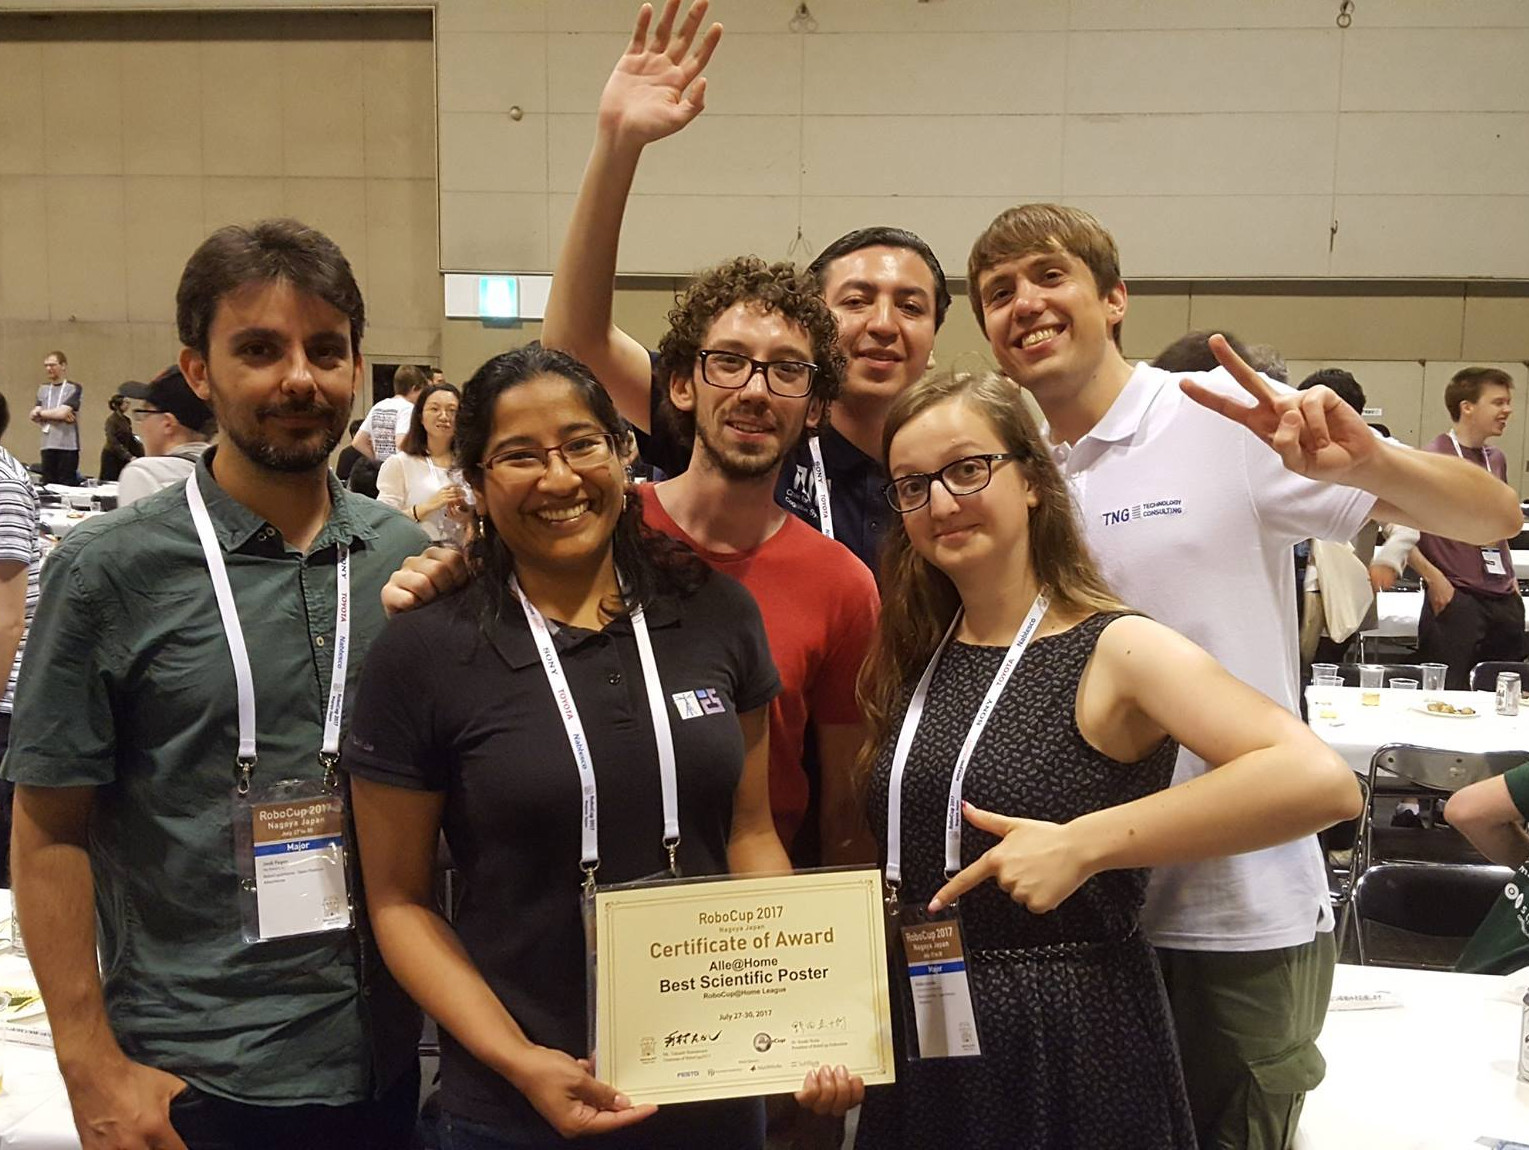
\includegraphics[width=\columnwidth]{../img/certificate.jpg}
        \caption{Best scientific poster certificate}
        \label{certificate}
    \end{figure}

    During the competition, we faced a total of 14 other teams in our league : the RoboCup@Home2017 Open Platform League. Most of them (if not all of them) were not on their first trial. We tried to solve 3 challenges out of the 4 challenges in stage I and we ended up ranked 3 out of 15 in one of them (Storing groceries, see section I). We worked for three months on this project and our final ranking was 12 out of 15. We got the first place for the poster presentation (see appendix \ref{appendix:poster}) in our league and we won the best scientific poster award, all leagues mixed up.

    Our code is open-source and will be released on github. The result of my internship is the perception module. A part of it (the recognition on an RGB image and the election server) is a standalone python library. It is easy to use in a different project: I used it on two separate platforms without changing the library itself.

    \begin{figure}[!b]
        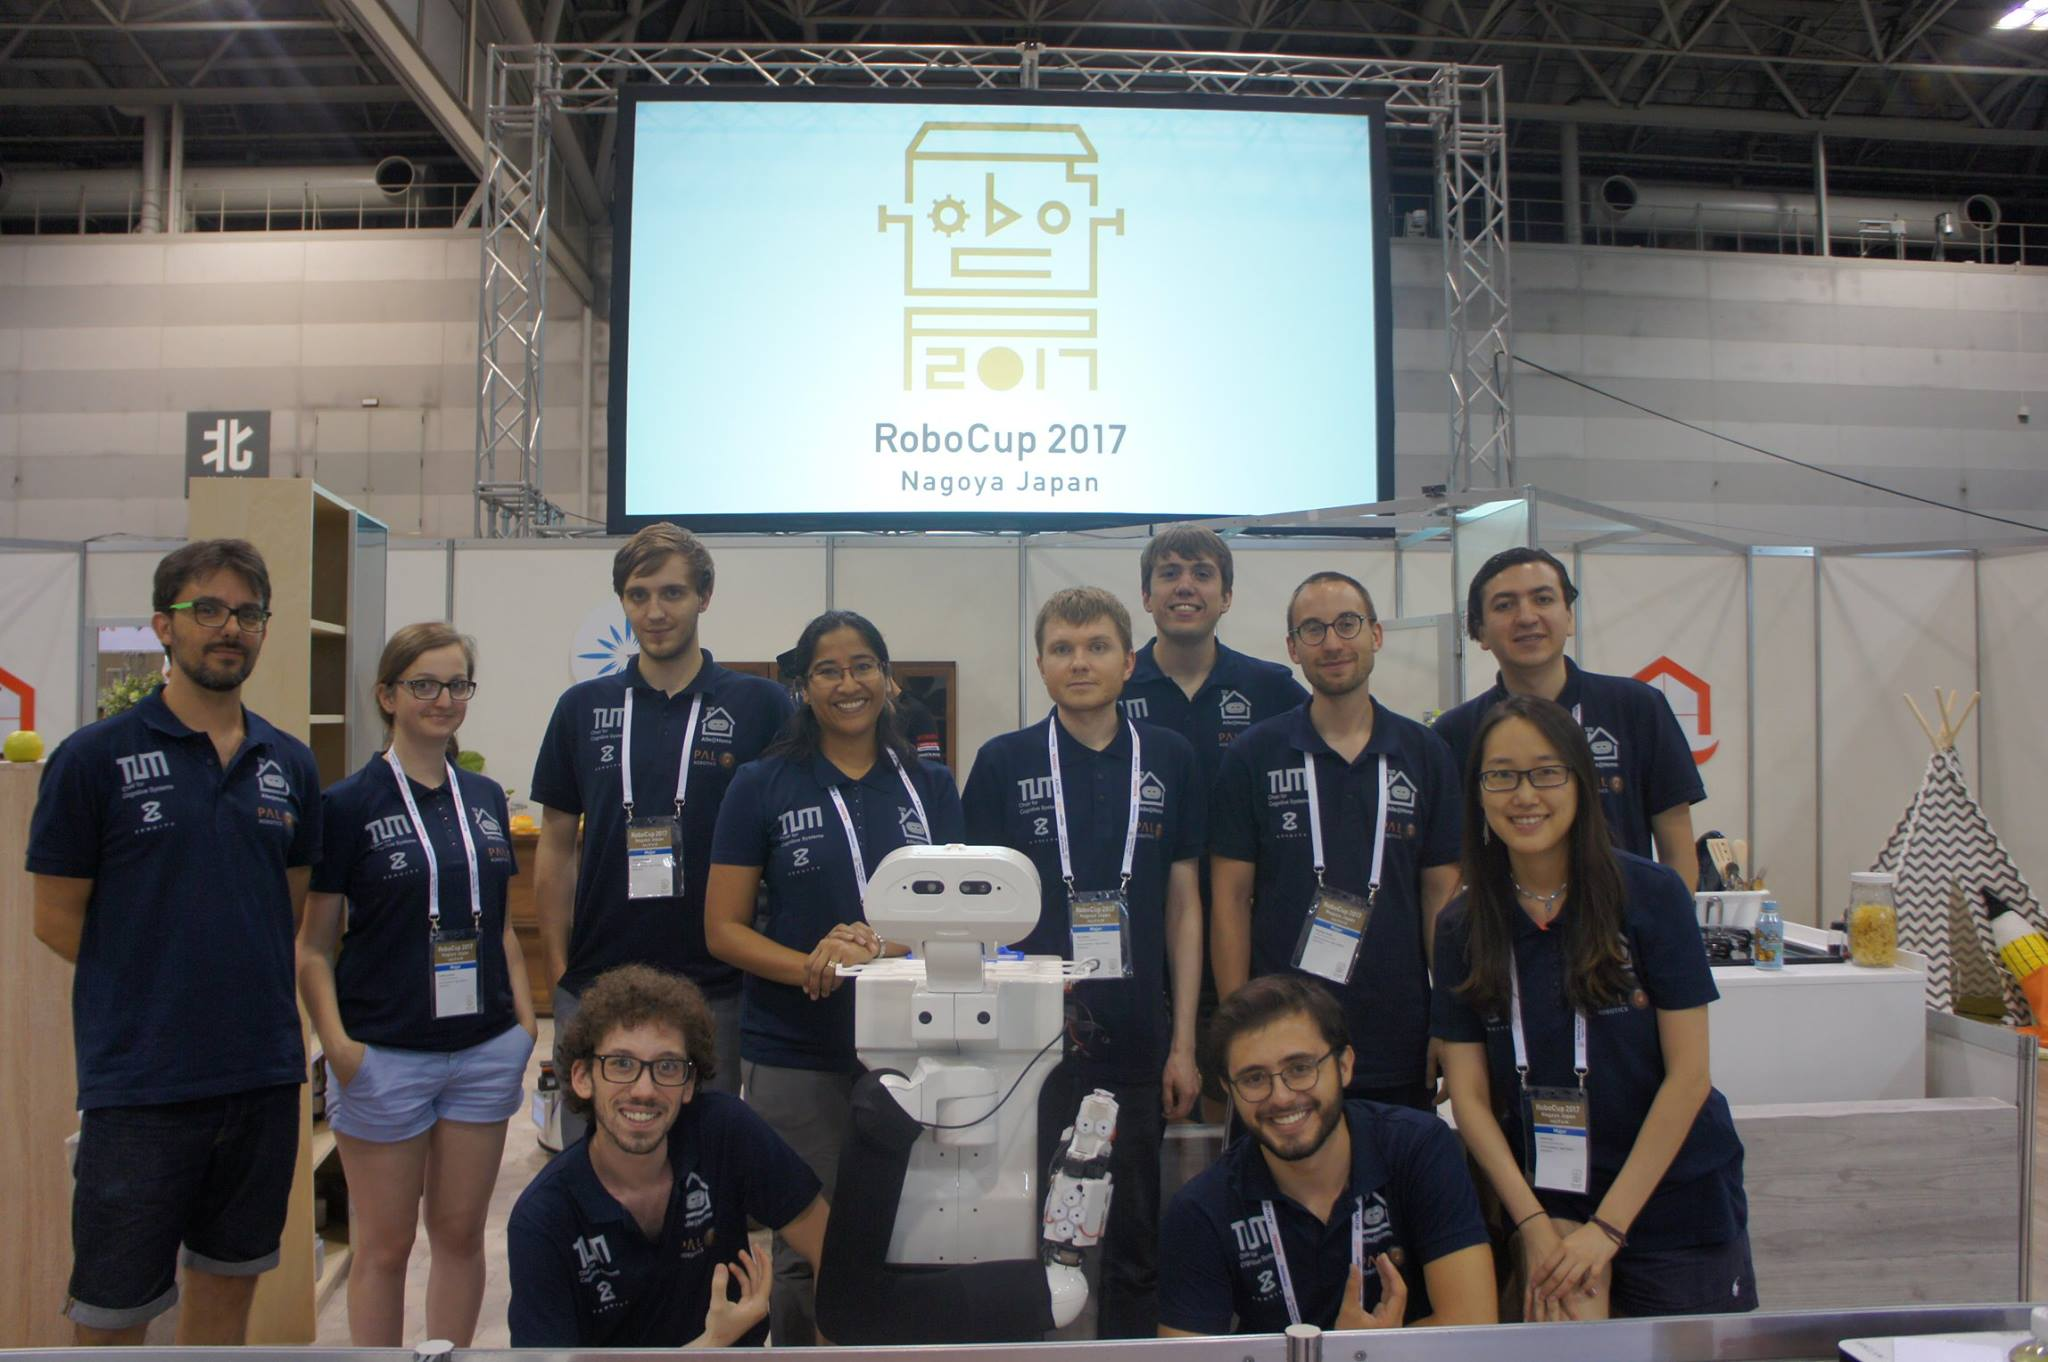
\includegraphics[width=\columnwidth]{../img/team.jpg}
        \caption{Part of our team}
        \label{team}
    \end{figure}

    \section*{Acknowledgments}

    I would like to thank Dr. Pablo Lanillos for his expert advice and help throughout this difficult project, as well as Germ\'{a}n D\'{i}ez Valencia for his wonderful collaboration. You supported me greatly and were always willing to help. Thanks to Patrick Grzywok, Emilka Skurzy\'{n}ska and the rest of the team for their friendship in the lab. Finally, thanks to Dr. Karinne Ram\'{i}rez-Amaro for her supervision and her encouragement. This project would not have been impossible without the support of TUM, PAL Robotics, TNG and our other sponsors.

    \vfill

    % ---------- R�f�rences

	\pagebreak

	\twocolumn[{\begin{@twocolumnfalse}
		\bibliographystyle{plain}
		\bibliography{report}
	\end{@twocolumnfalse}}]

    % ---------- Annexe
    \appendixpageoff

    \begin{appendices}
        \centering\noindent
        
        % Poster
        \twocolumn[{\begin{@twocolumnfalse}
            \subsection{Poster}
            \includegraphics[width=\textwidth]{poster.pdf}
            \label{appendix:poster}
        \end{@twocolumnfalse}}]

    \end{appendices}

\end{document}
